% (The MIT License)
%
% Copyright (c) 2023-2025 Yegor Bugayenko
%
% Permission is hereby granted, free of charge, to any person obtaining a copy
% of this software and associated documentation files (the 'Software'), to deal
% in the Software without restriction, including without limitation the rights
% to use, copy, modify, merge, publish, distribute, sublicense, and/or sell
% copies of the Software, and to permit persons to whom the Software is
% furnished to do so, subject to the following conditions:
%
% The above copyright notice and this permission notice shall be included in all
% copies or substantial portions of the Software.
%
% THE SOFTWARE IS PROVIDED 'AS IS', WITHOUT WARRANTY OF ANY KIND, EXPRESS OR
% IMPLIED, INCLUDING BUT NOT LIMITED TO THE WARRANTIES OF MERCHANTABILITY,
% FITNESS FOR A PARTICULAR PURPOSE AND NONINFRINGEMENT. IN NO EVENT SHALL THE
% AUTHORS OR COPYRIGHT HOLDERS BE LIABLE FOR ANY CLAIM, DAMAGES OR OTHER
% LIABILITY, WHETHER IN AN ACTION OF CONTRACT, TORT OR OTHERWISE, ARISING FROM,
% OUT OF OR IN CONNECTION WITH THE SOFTWARE OR THE USE OR OTHER DEALINGS IN THE
% SOFTWARE.

\documentclass{article}
\usepackage{../lecture-notes/notes}
\newcommand*\thetitle{Lines of Code (LoC)}
\begin{document}

\lnTitlePage{1}{24}{q9Gr2xguP5I}

\lnThought{Quality of code means \ul{maintainability}: how quickly other programmers can understand your code.}

\lnQuote
  {edsger-dijkstra}
  {It has been suggested that there is some law of nature telling us that the amount of intellectual effort needed grows with the \ul{square} of program \ul{length}. But, thank goodness, no one has been able to prove this law. And this is because it \ul{need not be true}.}
  {dijkstra1972humble}

\lnQuote
  {lionel-deimel}
  {One of the most overlooked programming skills is the ability to \ul{read} a program, an activity the programmer is called upon to do with surprising \ul{frequency}.}
  {deimel1985uses}

\lnQuote
  {../01-lines-of-code/darrell-raymond}
  {Whatever approach is used, it is clear that a central activity in software maintenance is \ul{reading}. In maintenance, the main role of source code is not as a compilable entity, but as a human-readable statement of the intent and mechanism of the program.}
  {raymond1991reading}

\lnQuote
  {fred-brooks}
  {A programmer depends upon other people's programs. These are often \ul{maldesigned}, \ul{poorly implemented}, \ul{incompletely delivered} (no source code or test cases), and \ul{poorly documented}. So he must spend hours studying and fixing things that in an \ul{ideal world} would be complete, available, and usable.}
  {brooks1995mythical}

\lnQuote
  {harold-abelson}
  {We want to establish the idea that a computer language is not just a way of getting a computer to perform operations but rather that it is a novel \ul{formal medium} for expressing ideas about methodology. Thus, programs must be written for people to read, and only \ul{incidentally} for machines to execute.}
  {abelson1996structure}

\lnQuote
  {robert-martin}
  {Indeed, the ratio of time spent reading vs. writing is well over 10:1. We are constantly reading old code as part of the effort to write new code. Because this ratio is so high, we want the \ul{reading} of code to be easy, even if it makes the \ul{writing} harder.}
  {martin2008clean}

\lnQuote
  [Dustin Boswell]
  {dustin-boswell}
  {Code should be written to minimize the \ul{time} it would take for someone else to understand it. It's so important that we call it The Fundamental Theorem of Readability.}
  {boswell2011art}

\lnThought{Everybody wants higher \ul{quality of code}, but nobody knows how to measure it.}

\lnQuote
  {shari-lawrence-pfleeger}
  {It's not enough to make claims about your software; you must support your claims with \ul{measurable evidence}.}
  {pfleeger2008software}

\lnQuote
  [Mariza A. S. Bigonha]
  {mariza-bigonha}
  {The application of \ul{thresholds} could lower the cost of software quality evaluation since they can reduce the amount of software code that should be inspected. Therefore, the thresholds provide a way for quantitative and qualitative evaluations to complement each other, leading to a more efficient quality \ul{assessment} of object-oriented software systems.}
  {filo2024evaluating}

\lnPitch{
  \begin{multicols}{2}
  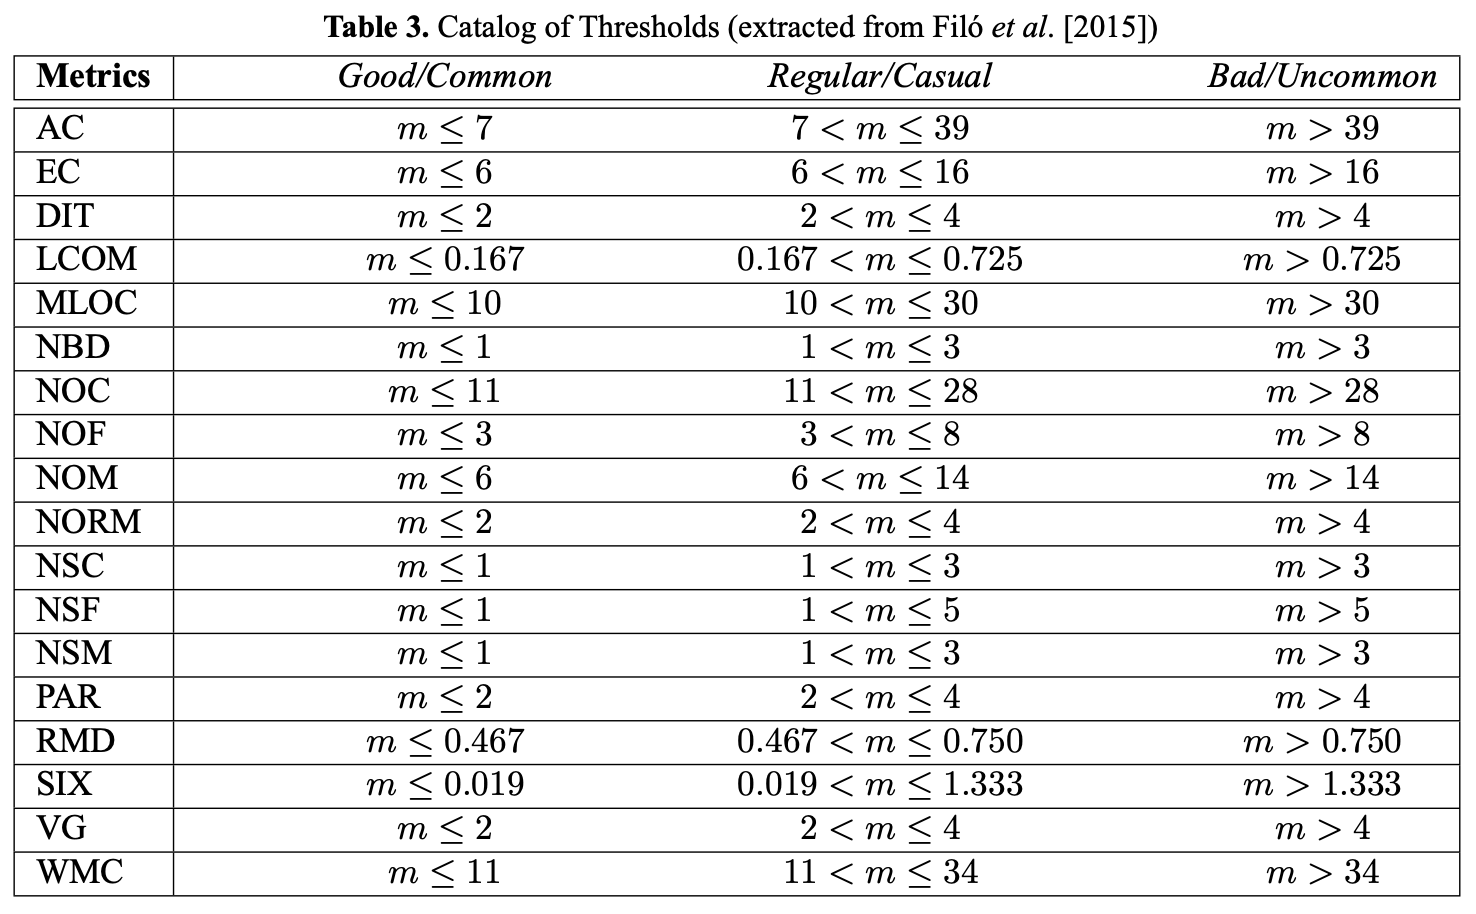
\includegraphics[width=.95\linewidth]{thresholds.png}
  \par\columnbreak\par
  To evaluate our catalog, in that work, we handled a case study to assess proprietary software from a public organization with a bad internal quality to verify the proposed thresholds' ability to indicate it.\par
  \lnSource{filo2024evaluating}\par
  \lnSource{filo2015catalogue}
  \end{multicols}}

\lnThought{Size of code is the key contributor to its quality, while Lines of Code (LoC) is the basic measurement of size.}

\lnQuote
  {steve-mcconnell}
  {Studies have found that larger routines are more \ul{error-prone} than smaller ones. Keeping routines short helps reduce errors and makes the code easier to maintain.}
  {mcconnell2004code}

\lnQuote
  {robert-martin}
  {The first rule of functions is that they should be \ul{small}. The second rule of functions is that they should be even \ul{smaller} than that.}
  {martin2008clean}

\lnThought{It \ul{may} be wrong to measure productivity of a programmer by counting lines of code, but for the quality of code the LoC metric is a perfect indicator.}

\lnPitch{
  \pptBanner{\texttt{cloc.pl}}
  \pptPic{.65}{cloc.png}\par
  \url{https://github.com/AlDanial/cloc}}

\lnThought{In 2011, Uncle Bob \href{https://softwareengineering.stackexchange.com/questions/66523}{suggested} that 200 lines per Java class is a good guideline to stay below.}

\lnPitch{
  \begin{multicols}{2}
  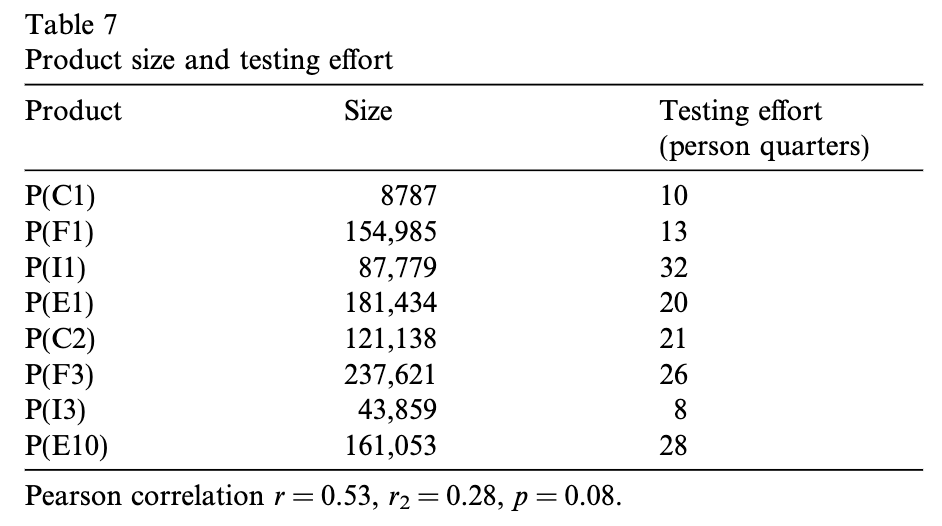
\includegraphics[width=\linewidth]{size-vs-testing.png}
  \par\columnbreak\par
  ``We conclude that code size is not a good predictor of testing effort (measured by allocated test engineers) at either product or product line levels. Other metrics, like code coupling and cohesion are more appropriate for such estimation.''\par
  \lnSource{ajila2007experimental}
  \end{multicols}}

\lnThought{Instead of counting lines, it may be more reasonable to count NCSS (Non Commenting Source Statements), but not always.}

\pptBanner{LoC vs NCSS}
\begin{multicols}{2}
{\small\begin{ffcode}
#!/bin/bash
set -e

# Simple intro:
printf "Hello, %s!
  Your balance is %d." \
  "${name}" \
  "$(psql 'SELECT balance
    FROM user WHERE id = 42')"
\end{ffcode}
}
\par\columnbreak\par
Lines of Code = ?
\par
NCSS = ?
\end{multicols}
\plush{}

\lnThought{There are \href{https://www.linux.com/news/linux-in-2020-27-8-million-lines-of-code-in-the-kernel-1-3-million-in-systemd/}{27.8M} lines of C code in Linux kernel. What does it tell us?}

\lnPitch{
  \pptBanner{Largest Open Source Projects}
  \begin{multicols}{2}
  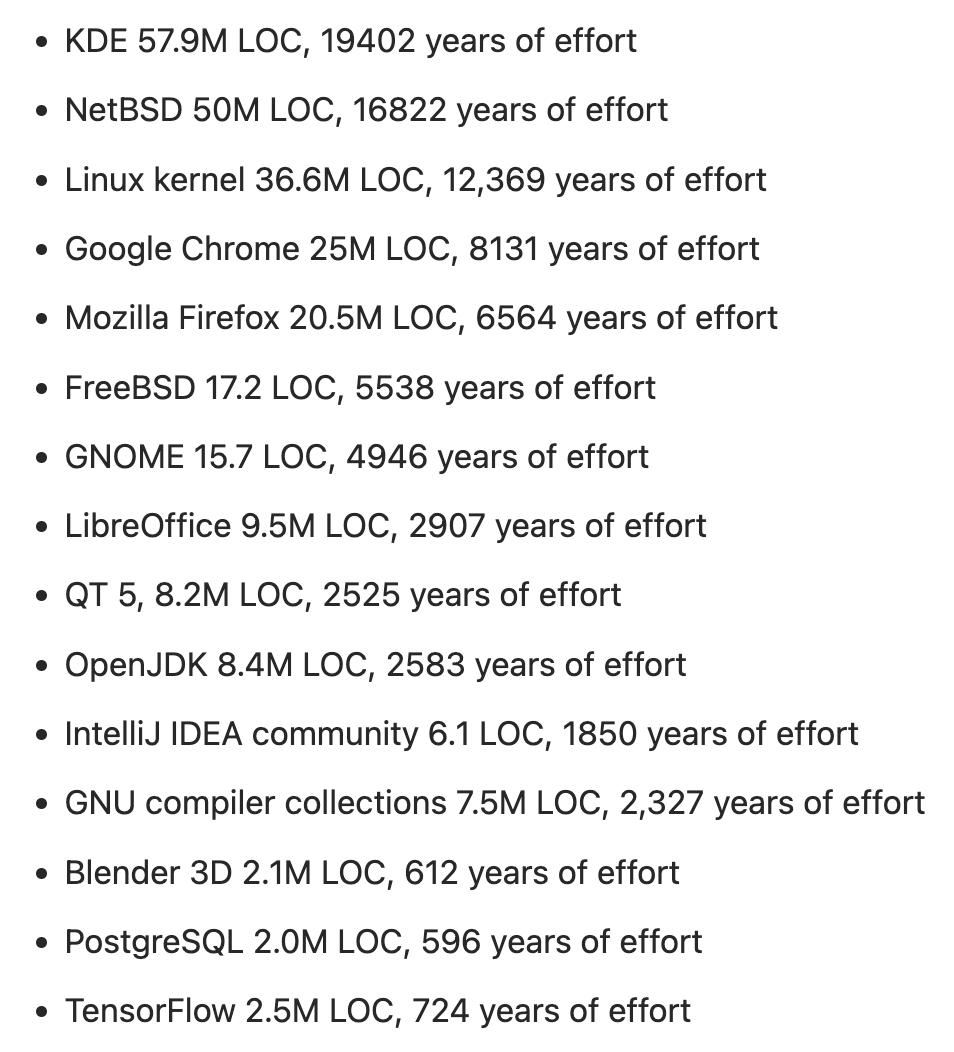
\includegraphics[width=.8\linewidth]{largest.png}\par
  {\scriptsize Found it on \href{https://www.quora.com/What-are-some-open-source-projects-with-the-largest-complexity-by-lines-of-code-or-developer-effort/answer/Felix-Zaslavskiy}{Quora}.\par}
  \par\columnbreak\par
  How many lines of code are in your repositories?
  How many lines of code you write every week?
  How many lines of code you delete every week?
  How about annually?
  \end{multicols}}

\lnThought{Java is \href{http://jameshfisher.github.io/languageredundancy/}{two times} more verbose than Ruby. Does it mean the quality of an average Ruby code is higher?}

\end{document}
